\chapter{\chImplementation}
\label{ch:implementation}

\section{System Design}

\subsection{Architecture}

\begin{figure}
    \centering
    \makeatletter
\tikzset{
    database/.style={
        path picture={
            \draw (0, 1.5*\database@segmentheight) circle [x radius=\database@radius,y radius=\database@aspectratio*\database@radius];
            \draw (-\database@radius, 0.5*\database@segmentheight) arc [start angle=180,end angle=360,x radius=\database@radius, y radius=\database@aspectratio*\database@radius];
            \draw (-\database@radius,-0.5*\database@segmentheight) arc [start angle=180,end angle=360,x radius=\database@radius, y radius=\database@aspectratio*\database@radius];
            \draw (-\database@radius,1.5*\database@segmentheight) -- ++(0,-3*\database@segmentheight) arc [start angle=180,end angle=360,x radius=\database@radius, y radius=\database@aspectratio*\database@radius] -- ++(0,3*\database@segmentheight);
        },
        minimum width=2*\database@radius + \pgflinewidth,
        minimum height=3*\database@segmentheight + 2*\database@aspectratio*\database@radius + \pgflinewidth,
    },
    database segment height/.store in=\database@segmentheight,
    database radius/.store in=\database@radius,
    database aspect ratio/.store in=\database@aspectratio,
    database segment height=0.1cm,
    database radius=0.25cm,
    database aspect ratio=0.35,
}
\makeatother

\tikzstyle {block} = [draw, text width=4cm, minimum height=1cm, align=center]
\tikzstyle {miniblock} = [draw=gray, dashed, text width=3cm, inner sep=1ex]

\begin{tikzpicture}
    \node [block] (bootstrapper) {Bootstrapper};
    \node [block, below=of bootstrapper] (manager) {Manager};
    \node [block, below=1.5cm of manager, inner sep=0pt] (worker) {
        \begin{tikzpicture}
            \matrix [row sep=1em] {
                \node {Worker}; \\
                \node [miniblock] {\footnotesize Collect System Info}; \\
                \node [miniblock] {\footnotesize Execute run}; \\
                \node [miniblock] {\footnotesize Validate result}; \\
                \node {\dots}; \\
            };
        \end{tikzpicture}
    };
    \draw [-latex'] (manager) -- (worker) node [midway, fill=white] {manages};

    \node [block, right=3cm of bootstrapper, inner sep=0pt] (server) {
        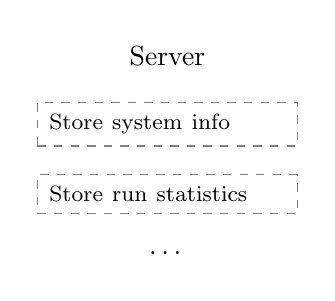
\begin{tikzpicture}
            \matrix [row sep=1em] {
                \node {Server}; \\
                \node [miniblock, outer sep=2ex] {\footnotesize Store system info}; \\
                \node [miniblock, outer sep=2ex] {\footnotesize Store run statistics}; \\
                \node {\dots}; \\
            };
        \end{tikzpicture}
    };
    \node[database,database radius=0.5cm,database segment height=0.3cm, below=of server] (database) {};
    \node [right=0.1cm of database] {\rotatebox{-90}{Database}};
    \node [block, below=of database, inner sep=0pt] (analyzer) {
        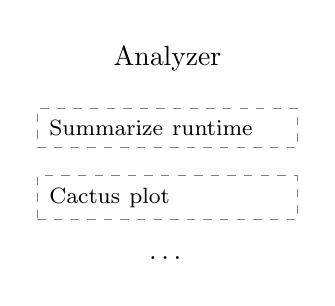
\begin{tikzpicture}
            \matrix [row sep=1em] {
                \node {Analyzer}; \\
                \node [miniblock] {\footnotesize Summarize runtime}; \\
                \node [miniblock] {\footnotesize Cactus plot}; \\
                \node {\dots}; \\
            };
        \end{tikzpicture}
    };
    \draw (server) -- (database);
    \draw (database) -- (analyzer);

    \draw [-latex'] (bootstrapper) -- (server) node [midway, fill=white] {$R \in C \times I$};
    \path [-latex', transform canvas={yshift=0.2cm}] (server) edge node [sloped, above, pos=0.33, fill=white] {$(c,i) \in R$} (worker);
    \path [-latex', transform canvas={yshift=-0.2cm}] (worker) edge node [sloped, below, pos=0.33, fill=white] {reports to} (server);

    \begin{scope}[on background layer]
        \node[draw=red!50, dashed, inner sep=1ex, label=above:\sffamily\textsc{client-side},  rounded corners, fit=(bootstrapper)(manager)(worker)] (clientenv) {};
        \node[draw=blue!50, dashed, inner sep=1ex, label=above:\sffamily\textsc{server-side},  rounded corners, fit=(server)(database)(analyzer)] (serverenv) {};
        \path [draw=black!30, dashed] ([xshift=-1.5cm] serverenv.north west) edge node [sloped, near end, text=black!60, fill=white] {TCP} ([xshift=-1.5cm] serverenv.south west);
    \end{scope}

\end{tikzpicture}

    \caption{Architecture of \OurBenchmarkingTool}
    \label{fig:architecture}
\end{figure}

Figure \ref{fig:architecture} shows the architecture of \OurBenchmarkingTool, our attempt on a new benchmarking tool fulfilling most of the defined requirements.
The architecture follows the client-server design pattern, communicating through Transmission Control Protocol (TCP).
The client manages the heavy computation while the server manages the data.
Typically, the client will be in a high performance computing (HPC) cluster system while the server in a separate system---e.g. a virtual private server (VPS)---to avoid long running jobs.

\emph{Server} manages the data in the database.
It receives events through a TCP socket and optionally send replies.
To achieve extensibility, the server maintains a specified set of \emph{observers}, each listening for related events.
The events are distributed through a publisher-subscriber design pattern.
The observer will then executes its jobs, such as inserting data to the database.

\emph{Bootstrapper} is a component that will read the configuration file from the user, prepare the computing environment, and then tell the server $R \in C \times I$, the set of benchmark runs that will be executed.
Among the things prepared are the tools, benchmark instances, and database schema.
Preparing the specified tools and instances may additionally include downloading and running related setting up steps.

\emph{Manager} manages the benchmark workers.
This component acts as an interface to the underlying job submitting system, or even implements its own job queue as in the case of the \emph{local} manager.
The manager is responsible for deploying, assigning tasks, and stopping the benchmark workers, making sure they finishes the assigned job.

\emph{Workers} do the heavy computing steps, typically in parallel.
Because the benchmark run is embarrassingly parallel\footnote{in other words, there is no dependencies between the tasks}, each worker can be run as its own process without interacting with other workers.
Submitted to a HPC cluster, this allows the computation to be executed as fast as possible.
A worker is assigned a run $r = (c, i) \in R$ and executes the needed steps for the benchmark run after asking the context from the server.
The run step is executed in sequence.
In most cases, one of these steps, called the \emph{executor}, acts as a resource monitor and executes the tool configuration $c$ with the instance $i$.
The executor then measures and limits the execution of the tool.
Finally, each step can report its result to the server.

\emph{Analyzer} aggregates the data from the database and analyze it, outputting a presentable result.
This component is usually used after the benchmarking is finished, but it can also be used to serve a live analysis of a benchmarking in process.
Analyzer is implemented as a module that can be reused by others.
This is to encourage code reuse and minimize the effort of doing the common analysis of research results.


\subsection{Network architecture}

\begin{figure}
    \tikzstyle{bidirectional} = [draw, latex'-latex']

\tikzset{
    pics/zmq2/.style n args = {3}{
        code = {
        \node[minimum height=3em, align=center] (-A) at (0,0) {#1};
        \node[fill=black!5, anchor=north east, text width=4em, align=center] (-B) at (-A.south) {\textsc{#2}};
        \node[fill=black!5, anchor=north west, text width=4em, align=center] (-C) at (-A.south) {\textsc{#3}};
        \node[inner sep=0pt,draw,rounded corners,fit=(-A)(-B)(-C)] {};
        \draw (-B.north west) -- (-C.north east)
              (-B.north east) -- (-C.south west);
        }
    },
    pics/zmq1/.style n args = {2}{
        code = {
        \node[minimum height=3em, align=center, text width=5em] (-A) at (0,0) {#1};
        \node[fill=black!5, anchor=north, text width=5em, align=center] (-B) at (-A.south) {\textsc{#2}};
        \draw (-B.north west) -- (-B.north east);
        \node[inner sep=0pt,draw,rounded corners,fit=(-A)(-B)] {};
        }
    },
}


\resizebox{\textwidth}{!}{%
    \begin{tikzpicture}
        \node (workerdots) {\huge\vdots};
        \pic [above=of workerdots, local bounding box=worker2] (w2) {zmq1={Worker 2}{dealer}};
        \pic [above=2cm of worker2, local bounding box=worker1] (w1) {zmq1={Worker 1}{dealer}};
        \pic [below=of workerdots, local bounding box=workern] (wn) {zmq1={Worker $m$}{dealer}};

        \pic [right=3cm of workerdots, local bounding box=server] (s) {zmq2={Gateway}{router}{pub}};

        \node [right=3cm of server] (observerdots) {\huge\vdots};
        \pic [above=of observerdots, local bounding box=observer2] (o2) {zmq1={Observer 2}{sub}};
        \pic [above=of observer2, local bounding box=observer1] (o1) {zmq1={Observer 1}{sub}};
        \pic [below=of observerdots, local bounding box=observern] (on) {zmq1={Observer $n$}{sub}};

        \path [bidirectional] (w1-B.east) -- (s-B.west);
        \path [bidirectional] (w2-B.east) -- (s-B.west);
        \path [bidirectional] (wn-B.east) -- (s-B.west);

        \path [bidirectional] (s-C.east) -- (o1-B.west);
        \path [bidirectional] (s-C.east) -- (o2-B.west);
        \path [bidirectional] (s-C.east) -- (on-B.west);

        \node [inner sep=.5cm, text=red!60!black, above, rotate=90, text width=4em] (w1label) at (worker1.west) {\sffamily\textsc{worker process}};
        \node [inner sep=.5cm, text=red!60!black, above, rotate=90, text width=4em] (w2label) at (worker2.west) {\sffamily\textsc{worker process}};
        \node [inner sep=.5cm, text=red!60!black, above, rotate=90, text width=4em] (wnlabel) at (workern.west) {\sffamily\textsc{worker process}};


        \begin{scope}[on background layer]
            \node[fit=(worker1)(worker2)(workerdots)(workern)] (workers) {};
            \node[fit=(observer1)(observer2)(observerdots)(observern)] (observers) {};

            \node[draw=red!50, inner sep=1ex, dashed, rounded corners, fit=(worker1)(w1label)] {};
            \node[draw=red!50, inner sep=1ex, dashed, rounded corners, fit=(worker2)(w2label)] {};
            \node[draw=red!50, inner sep=1ex, dashed, rounded corners, fit=(workern)(wnlabel)] {};
            \node[draw=blue!50, inner sep=2ex, dashed, rounded corners, fit=(server)(observers)] (serverenv) {};
        \end{scope}

        \node [inner sep=.5cm, text=blue!60!black, below right] at (serverenv.north west) {\sffamily\textsc{server process}};


    \end{tikzpicture}
}
    \caption{Network architecture}
    \label{fig:zmq}
\end{figure}


\subsection{Benchmarking Workflow}
\subsection{Design Rationale}



\begin{figure}
    \centering
    \includegraphics[width=\textwidth]{assets/pics/workflow-swimlane.png}
    \caption{Benchmarking workflow}
\end{figure}

\section{Implementation}
\section{Usage Scenario}
